\section{Closed form}

L'idea di poter definire un sotto-linguaggio per ciauscun simbolo è molto comodo perchè posso partire da un linguaggio e usare quello.
Il linguaggio prodotto è il prodotto dei linguaggi, la production independent è una cosa che utilizziamo molto.
Le context-free consentono una struttura che viceversa perdiamo se andiamo nel linguaggi regolari ed è la questione del self embedding.

\subsection{Self embedding}
Si intende come regola ricorsiva quando nel lato destro della produzione compare il simbolo non terminale che si sta definendo:
\begin{align*}
    A &\to aAa
\end{align*}

La regola ricorsiva è l'ingrediente necessario per rendere i nostri linguaggi infiniti.
Questa regola ci serve ad esempio ad avere il linguaggio di Dyck, che è un linguaggio di parentesi ben formate.
\begin{align*}
    A &\to ( A ) 
\end{align*}
E questo ci porta a definire correttamente un linguaggio di programmazione.
Il Context-Free è un ragionevole punto di incontro tra un linguaggio regolare e un linguaggio ricorsivo (basso ed alto livello).

\section{Alberi di parsing}
L'albero cattura la forma gerarchica di un linguaggio, è un modo per rappresentare la struttura di un linguaggio. Sia a fini linguistici sia per rappresentare la struttura di un linguaggio di programmazione.

Prima di poterci dedicare in maniera serena a questi alberi di parsing dobbiamo fare un po' di pulizia perchè abbiamo delle grammatiche con difetti che vorremmo eliminare. La spazzatura che può rimanere dentro una gramamtica context free è che possiamo avere dei non terminali non definiti. Cioè abbiamo messo dentro delle variabili (lettere maiuscole) che non abbiamo definito, non stanno mai a sinistra di una produzione. Questo è un problema perchè non possiamo mai terminare la produzione. Sono inutili e vanno eliminati. Ci sono altre due circostanze in cui ci sono problemi, potremmo avere definito un terminale che non è mai raggiungibile da nessuna produzione, questi si chiamano \underline{simboli irraggiungibili} e vanno eliminati. Infine potremmo avere una produzione ricorsiva ma in questo caso non possiamo mai avere una produzione vuota con questa variabile, questa si chiama variabile improduttiva e va eliminata.
Un'altra circostanza non bella è avere un loop per derivare delle variabili.

\subsection{Pulizia di una grammatica}
\begin{enumerate}
    \item Eliminare i non terminali non definiti
    \item Eliminare i simboli irraggiungibili
    \item Eliminare le variabili improduttive
    \item Eliminare i loop
\end{enumerate}

Quello che chiediamo è che una variabile sia derivabile non subito ma dopo un numero n di passi. Quello che chiadiamo è una /underline{chiusura della funzione}, dato un insieme applico f in modo ricorsivo e se questa f è chiusa significa che prima o poi arrivo ad un insieme tale per cui se applico ancora la funzione a quell'insieme rimango in quell'insieme. Un esempio di funzione chiusa è se aumento sempre gli oggetti dell'insieme ma gli oggetti fanno parte di un insieme finito.

Dentro liblet c'è un decoratore @closure che ci permette di fare la chiusura di una funzione. \'E chiaro che con una funzione di questo tipo la pulizia diventa abbastanza semplice. Vediamo un esempio di una grammatica sporca:
\begin{lstlisting}
G = Grammar.from_string("""
S -> A B | D E
A -> a
B -> b C
C -> c
D -> d F 
E -> e 
F -> f D
""")
G
\end{lstlisting}

Le regole produttive si possono definire, in modo bottom up detrmino le produttive, deiventa produttivo a sinistra quello che a destra ha tutte cose produttive:
\begin{lstlisting}
def find_productive(G):

  @closure
  def find(prod):
    return prod | {A for A, a in G.P if set(a) <= prod}

  return find(G.T)

find_productive(G)
\end{lstlisting}

Le raggiungibili invece si possono ottenere con un processo top down, parto dal simbolo distinti e metto dentro tutti i non terminali a quali posso arrivare da qualcosa di raggiungibile:

\begin{lstlisting}
from liblet import union_of

def find_reachable(G):

  @closure
  def find(reach):
    return reach | union_of(set(a) for A, a in G.P if A in reach)

  return find({G.S})

find_reachable(G)
\end{lstlisting}

Dopo aver definito questo posso pulire la grammatica, garantisco che tutti i simboli sono produttivi e raggiungibili:
\begin{lstlisting}
def remove_unproductive_unreachable(G):
    Gp = G.restrict_to(find_productive(G))
    return Gp.restrict_to(find_reachable(Gp))

remove_unproductive_unreachable(G)
\end{lstlisting}

Attenzione che l'ordine con cui si fa questa operazione è cruciale, se eliminiamo prima i non non raggiungibili e poi i non produttivi potrei avere la necessità di dover fare un'altra passata per elminiare altri non raggiungibili.

\subsection{Dimensione degli alberi di parsing}
Ha senso ragionare sulla dimensione degli alberi di parsing? si perchè se fossero enormi non avrebbero una utilità pratica. La storia è molto semplice ed è legata al fatto che in buona sostanza la frontiera di un albero binario è lineare nel numero di nodi con N nodi abbiamo O(N) foglie. Quindi quello che vogliamo dimostrare che se prendiamo una grammatica non malata un albero di derivazione non può contenere più di N nodi.
Quello che facciamo è raginare bottomup, tutte le volte che vengo verso l'alto e faccio un passo agglomerativo (agglomero con un non terminale) un nodo lo aggiungo ma almeno due ne tolgo, il che vuol dire che se questa cosa allora ho introdotto N nodi e ne ho tolti 2N quindi ho inserito linearmente N nodi. Le cose che mi restano da guardare è cosa succede nel caso di regole unitarie, avendo regole unitarie al massimo si va ad esplodere nella dimensione dei non terminali, perchè significa che arrivo ad un agglomeratore tramite una catena.

\subsection{Derivazioni}
Non è detto che una parola derivata abbia sempre la stessa derivazione, ci sono tante derivazioni possibili da una grammatica per la stessa parola. Le derivazioni in termini di alberi di parsing vediamo che per due derivazioni diverse abbiamo lo stesso albero di parsing ed è una situazione spiacevole perchè ci sarebbe piaciuto avere una mappa 1-1, la presenza di più derivazioni più essere più o meno critica a seconda del contesto. Ci possono essere due derivazioni che hanno due alberi di parsing diversi che è la situazione che ci preoccupa, il primo caso è facilmente risolvibile indicando delle derivazioni preferibili (nel primo caso abbiamo per finta più derivazioni perchè alla fine cambia solo l'ordine).
Nel secondo caso abbiamo più alberi di parsing per più derivazioni.

\begin{lstlisting}
#  una grammatica banale per il linguaggio {a and nb | n > 0}

G_ab = Grammar.from_string('''
S -> A B
A -> a A | a
B -> b
""")
G_ab

# due possibili derivazioni

ab_0 = Derivation(G_ab).step(
  [(0, 0), (1,0), (2,1), (3,2)]
)
ab_1 = Derivation(G_ab).step(
  [(0, 0), (3,1), (1,0), (2,1)]
)

ab_0, ab_1

# ma a ben guardare lo stesso albero 

side_by_side(
  ProductionGraph(ab_0),
  ProductionGraph(ab_1),
)
\end{lstlisting}

\subsection{Dalla derivazione all'albero di parsing}
Cominciamo a ragionare sul fatto che non è così ovvio il legame tra le parole, le derivazioni e gli alberi di parsing.
Adesso cerchiamo di convincerci che almeno uno di questi pezzi è facilmente raggiungibile, esiste un modo semplice data una derivazione costruire un albero di parsing. Con Python posso tenermi la forma sentenziale conservando tutti gli aberi che mano a mano da questa forma sviluppo, la prima forma è il simbolo distinto e poi per ogni passo di derviazione mi dice quale pezzo della forma sentneziale va sostituito e noi sostituiamo questa con un nodo nell'albero.
Sostanzialmente per ogni passaggio di derivazione sostituisco mettendo i nodi nell'albero, nella forma sentenziale tengo sempre le foglie e sopra metto da dove derivo.
La seguente procedura memorizza in tree l'albero di derivazione e in frontier la sua frontiera, corrispondente alla forma sentenziale a cui è giunta la derivazione (di passo in passo) come una lista di alberi annotati.

Ciascun nodo dell'albero ha due etichette: Symbol che si riferisce ad uno dei simboli della grammatica e prord pari ad una produzione. I figli di ciascun nodo dell'albero hanno i simboli contenuti nel lato destro di prord.

Gli alberi vengono "completati" man mano che la procedura elabora i passi della derivazione; al termine le foglie degli alberi saranno simboli terminali (e prord sarà convenzionalmente definito come None).
\begin{lstlisting}
 def derivation_to_parsetree(d):

    # questa variabile si riferira all'albero di derivazione di d
    # inizialmente contiene l'albero annotato col simbolo di partenza
    tree = Tree({'Symbol': d.G.S, 'prod': None})

    # all'inizio la forma sentenziale e data da tale albero
    frontier = [tree, ] 

    for nprod, pos in d.steps():

        # l'albero da completare e dato dalla posizione in cui e applicata la produzione
        curr = frontier[pos]

        # risalgo dal numero alla produzione
        prod = d.G.P[nprod]

        # i figli sono dati dal lato destro d.G.P[prod].rhs
        children = [Tree({'Symbol': X, 'prod': None}) for X in prod.rhs]
        
        # aggiorno l'albero da completare
        curr.root['prod'] = prod
        curr.children = children

        # aggiorno la forma sentenziale
        frontier = frontier[:pos] + children + frontier[pos + 1:]

    return tree
\end{lstlisting}

Per tornare indietro (dall'albero alla derivazione) posso fare una visita in pre-ordine arriviamo ad una derivazione left most:
\begin{lstlisting}
 def leftmost(tree):
  return [tree.root['prod']] + [prod for child in tree.children for prod in leftmost(child) if prod] 
    
lm_0 = leftmost(pt_0)
lm_0
\end{lstlisting}

Da notare che se facciamo una visita in post-ordine non otteniamo una right most, ma una right most al contrario. Questo tipo di ambiguità è ineliminabile.
Questo è logicamente un problema quando abbiamo operatori non associativi (es. sottrazione e divisione).

Quello che dovremo fare quando scriveremo una grammatica:
\begin{enumerate}
    \item Non è sempre possibile
    \item Non è automatico
    \item Introduco N non "semantici": è chiaro che poi questi N andranno eliminati perchè producono alberi di parsing pieni di mondezza
\end{enumerate}

\subsection{Possibili soluzioni}
La ricorsione a sinistra determina un associatività a sinistra mentre se è a destra si usa una ricorsione a destra. Quello che facciamo e' inserire dei simboli in piu' nel linguaggio per gestire tutti i casi:

\begin{lstlisting}
  G_la = Grammar.from_string("""
  E -> E + E' | E'
  E' -> n 
  """)
  G_la
\end{lstlisting}
\begin{lstlisting}
  G_ra = Grammar.from_string("""
  E -> E' ^ E | E'
  E' -> n 
  """)
  G_ra
\end{lstlisting}
\newpage

\begin{figure}[ht!]
  \centering
  \begin{subfigure}{0.45\textwidth}
      \centering
      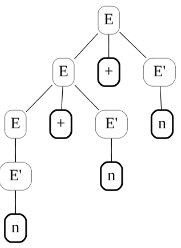
\includegraphics[scale=1]{images/AlberiParsing/associativitaSinistra.png}
      \caption{Associatività Sinistra}
  \end{subfigure}
  \hfill
  \begin{subfigure}{0.45\textwidth}
      \centering
      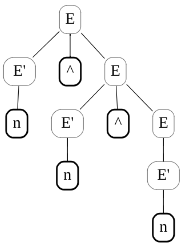
\includegraphics[scale=1]{images/AlberiParsing/associativitiaDestra.png}
      \caption{Associatività Destra}
  \end{subfigure}
  \caption{Confronto tra associatività sinistra e destra}
\end{figure}
 
Quando ho la menata della precedenza, operatori binari con precedenza diversa, questo si trdauce con l'introduzione di simboli ulteriori abbamo or n. Questi simboli sono terminali che rappresentano la precedenza degli operatori.

\begin{lstlisting}
  G_p = Grammar.from_string("""
  E -> E + P | P
  P -> P * F | F
  F -> n
  """)
\end{lstlisting}

\begin{figure}[ht!]
  \centering
  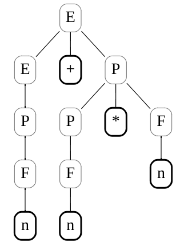
\includegraphics[scale=1]{images/AlberiParsing/precedenza.png}
\end{figure}

Nel caso del dangling else (if else if) diventa una cosa ancora più dolorosa c'è un interplate tra SMUC che è difficile da ricordare risolve la cosa perchè tiene l'else legato all'if più vicino.

\begin{lstlisting}
  G_if = Grammar.from_string("""
  S -> M | U
  M -> if C then M else M | stm
  U -> if C then M else U | if C then S
  C -> cond
  """)
\end{lstlisting}

\begin{figure}[ht!]
  \centering
  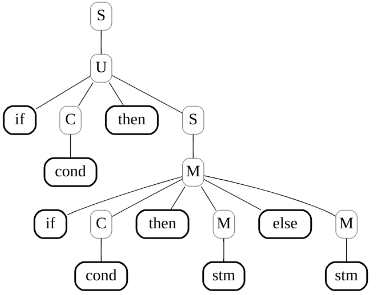
\includegraphics[scale=1]{images/AlberiParsing/dandlingElse.png}
\end{figure}

Il punto cruciale è che context free siamo al giusto livello (non ci siamo persi le parentesi sotto) abbiamo alberi di parsing lineari nella lunghezza della parola, ma dobbiamo stare attenti che avremo ambiguità ed in questo caso dobbiamo o modificare la grammatica che però sarà piena di non terminali e spesso questa procedura passa da trucchi e non c'è niente di teorico (che si possono copiare o inventare).
